\documentclass{ximera}

\title{Final Project Help: Classification with Gradient Descent}
\author{Zack Reed}

\begin{document}
\begin{abstract}
This page will help you as you work on your final project, exploring how to model classification problems using gradient descent. We'll begin with a simple linear classifier, then extend it to more complex models using calculus and optimization techniques.
\end{abstract}
\maketitle

\section*{Introduction}
For this final project we'll explore how to use \textbf{gradient descent} for \textbf{binary classification} using logistic regression. 

Unlike the Module 6 mini project where we approximated data with polynomials, classification separates data to distinguish between two options (yes/no, pass/fail, class 0/class 1).

\section*{Context: Binary Classification}
Many real-world problems involve predicting binary outcomes:
\begin{itemize}
  \item Medical diagnosis: is the disease present or not?
  \item Email filtering: is this message spam or legitimate?
  \item Student success: will the student pass or fail?
  \item Credit risk: will a loan default or be repaid?
\end{itemize}

For binary classification with features $(x_1, x_2)$, \textbf{logistic regression} uses the sigmoid function $\sigma(z) = \frac{1}{1+e^{-z}}$ to squish any real number into the range $[0,1]$.

We use the sigmoid to determine whether a point is on one side of a line $w_0 + w_1 x_1 + w_2 x_2 = 0$ (class 0) or on the other side of a line (class 1). 
The line separating the classes is called a \textbf{decision boundary}.

\begin{example}
Here is some sample data $(x_i, y_i)$ broken up into two classes:
\begin{itemize}
  \item Class 0 represented by blue circles
  \item Class 1 represented by red xs
\end{itemize}
In this example, we are given a line that separates the classes.
% \textbf{MATLAB code:}
% \begin{verbatim}
% [xy_demo, class_demo, coeffs_demo] = generate_classification_data(12345);
% plot_classification_data(xy_demo, class_demo, coeffs_demo);
% \end{verbatim}

\begin{center}
  \includegraphics{data_with_line.png}
\end{center}

As you can see, the data cleanly separated on either side of a line. 
\end{example}

The goal of this final project will be to use gradient descent to find \textbf{decision boundaries} in various scenarios for application in classification.

\begin{remark}
In this case, the \textbf{decision boundary} is a \textbf{line in 2D}, meaning it is represented by three parameters:
\begin{itemize}
  \item $w_0$, the constant
  \item $w_1$, the coefficient of $x$
  \item $w_2$, the coefficient of $y$
\end{itemize}

The goal of the gradient descent will be to minimize the error created by a line with these three parameters $(w_0, w_1, w_2)$. 

This gives us a line
\[
w_0 + w_1 x + w_2 y = 0
\]
that hopefully cleanly separates the data.
\end{remark}

\subsection*{Understanding the Sigmoid Function}
One key difference between the polynomials used in Module 6 and binary classification is the \textbf{sigmoid function}.

\[
\sigma(z) = \frac{1}{1+e^{-z}}
\]

This compresses all real numbers down to be between 0 and 1, so that we can use a height of $0.5$ to determine on which side of the line a data point lies.

If we measure the distance from the data points $(x_i, y_i)$ to the line $w_0 + w_1 x + w_2 y = 0$ (which you know how to do from back in Module 1), we get z-values into which we can use $\sigma$ to measure the location of the data relative to the line.

% The following cell shows how the sigmoid function is used in the separation decision.
% \textbf{MATLAB code:}
% \begin{verbatim}
% plot_sigmoid_values(xy_demo, class_demo, coeffs_demo)
% \end{verbatim}

\begin{center}
  \includegraphics{data_with_sigmoid.png}
\end{center}

In the left plot you see the distances from the line to the data points (keeping track of positive or negative) and then on the right you should see the resulting locations on the sigmoid plot, used to determine the class of the data.
The demo line very cleanly separated the classes, as you can see in the plot.

\subsection*{Poorly Separating Data}
Let's take a quick look at a line that doesn't separate the data, and see what happens to the sigmoid plot.
% \textbf{MATLAB code:}
% \begin{verbatim}
% coeffs_demo_2 = initialize_coefficients(xy_demo, class_demo);
% plot_sigmoid_values(xy_demo, class_demo, coeffs_demo_2);
% \end{verbatim}

\begin{center}
  \includegraphics{data_with_sigmoid_bad_separation.png}
\end{center}

Unlike the first line used in the demo, this line passes through the data points directly and so both sides of the line contain data from both classes. This means that the data is clustered on both sides of the sigmoid height $0.5$, so we can't use this line to determine between the classes.

\section*{Your Turn: Separating Personal Data}
You will generate your own data set that starts with a poor separator and then use gradient descent to improve it.

First, you will generate your data. In this walkthrough we will use the same data provided by default in the live script, with random seed 12345.

\begin{example}
The data given is the following 100 points separated evenly into two classes:

\begin{center}
  \includegraphics{data_no_line.png}
\end{center}

We again will start with a poor separator of the data, but will use gradient descent to improve it.

The randomly generated starting coefficients $(w_0, w_1, w_2)$ from the live script makes the vector \[\begin{bmatrix}
-0.131 \\
  0.344 \\
0.932
\end{bmatrix}\] which is the following vector in 3D space:

%make a 3D plot of the vector here

\begin{center}
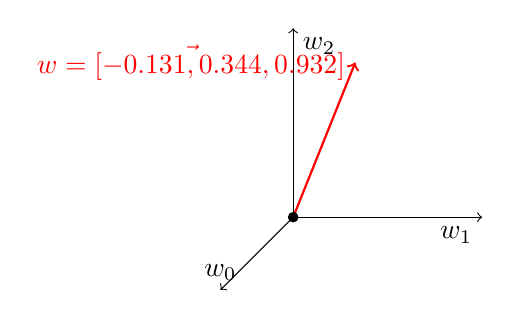
\begin{tikzpicture}[scale=2]
  % Axes
  \draw[->] (0,0,0) -- (1.2,0,0) node[anchor=north east]{$w_1$};
  \draw[->] (0,0,0) -- (0,1.2,0) node[anchor=north west]{$w_2$};
  \draw[->] (0,0,0) -- (0,0,1.2) node[anchor=south]{$w_0$};
  % Vector
  \draw[thick,red,->] (0,0,0) -- (.344, 0.932, -0.131) node[anchor= east]{$\vec{w=[-0.131, 0.344, 0.932]}$}; %(-0.131,0.344,0.932)
  % Origin
  \filldraw[black] (0,0,0) circle (0.03);
\end{tikzpicture}
\end{center}

This vector makes the line

\[-0.131 + 0.344 x + 0.932 y = 0\]

which poorly separates the data, as shown below:

\begin{center}
  \includegraphics{data_not_learned_bad_separation.png}
\end{center}

We measure how poor the separation is using the sigmoid function. In the following sigmoid plot, we see an accuracy of 35\%, meaning that only 35\% of the data points correctly lied above or below the height $\sigma (z) = 0.5$.

\begin{center}
  \includegraphics{predictions_not_learned.png}
\end{center}

\end{example}

% \textbf{MATLAB code:}
% \begin{verbatim}
% coeffs = initialize_coefficients(xy, class);
% for iter = 1:max_iters
%     coeffs = update_coefficients(xy, class, coeffs);
% end
% plot_sigmoid_values(xy, class, coeffs);
% \end{verbatim}

\subsection*{Gradient Descent: The Error Function (Binary Cross-Entropy)}

So far, we have auto-calculated the best line to use in the data separation problem. This separator is what can be learned in gradient descent, much like the polynomial fits to the data in Module 6.

To leverage gradient descent, however, we need an error function to be minimized. For reasons we won't get into, a standard error function for classification is \textbf{binary cross-entropy}:

\[L(w) = -\frac{1}{n} \sum_{i=1}^n \left[ c_i \log(p_i) + (1 - c_i) \log(1 - p_i) \right]\]

where  $p_i=\sigma(w_0 + w_1 x_i + w_2 y_i)$

is the sigmoid value aligned with the line for data point  

$(x_i, y_i)$ and $c_i$ is the actual class value (0 or 1) of the data point $(x_i, y_i)$.

Though the error function is somewhat complex, its gradients with respect to weights have a remarkably simple form:

\[\frac{\partial L}{\partial w_j} = \frac{1}{n} \sum_{i=1}^n (p_i - c_i) x_{ji}\]

If you look closely, you see that the gradient explicitly depends on the difference between $p_i$ and $c_i$, the error between the sigmoid output of the data point and the actual class value of the data point!

The term $x_{ji}$ is the  component of the the data point. (So $x_{2,100}$ is the y-component of the 100th data point).

That is, we can explicitly compute the gradients without taking derivatives of complicated functions, so we can directly employ gradient descent without complicated derivatives.

\subsection*{Gradient Descent for Classification}

Whereas the Module 6 activity ran gradient descent automatically, we will run gradient descent explicitly and then verify our results with a course function.


Remember that gradient descent works as follows:
\begin{enumerate}
  \item Randomly place points in the domain.
  \item Calculate the gradient of the function at the points.
  \item Move the points by subtracting a small multiple of the gradient
  
  \[ P_{n+1} = P_n - \alpha \nabla f(P_n) \]
  
  where $\alpha$ is a small positive number. We subtract because the gradient points in the direction of increase and we want to decrease.
  \item The points will stop moving eventually because when the gradients get small, the points will essentially be the same as before, and gradients get small at locations of critical points.
\end{enumerate}

We call $\alpha$ in step 3 the \textbf{learning rate} (step size). A standard value for $\alpha$ is $0.1$. We won't investigate its role very closely except to note that scaling down the gradients is what causes the points to actually slow down when they reach a local minimum.

\subsection*{Binary Cross Entropy Gradient Descent}

You are given an array called \texttt{classes} which the true class values of the data (0 or 1), so there is error between the values of calsses and the values of predictions.

Remember that the gradient of the binary-cross-entropy function is explicitly calculated from the partial derivatives.

\[\frac{\partial L}{\partial w_j} = \frac{1}{n} \sum_{i=1}^n (p_i - c_i) x_{ji}\]

Here, $n$ is the nubmer of data points and  is theth component of the th data point. The component matches the parameter .
Using this, we can proceed one parameter at a time to build the gradient function. 

Remember, the gradient $\nabla L=[L_x, L_y, L_z, \ldots]$ is the vector of partial derivatives. 
We have a way to compute each component of the error gradient function, so we will perform the gradient descent by doing the following:


\begin{enumerate}
  \item Create a random initial parameter point $P_0 = (w_0, w_1, w_2)$ that will be a "first guess" of the line to split the data.
  
  \item Split the data into three components, one per parameter of the line: $x_0$ (constant, usually a vector of ones), $x_1$ (the $x$-values), and $x_2$ (the $y$-values).
  
  \item Use a linear combination of the data components and the parameter components to make a vector of $z$-values for the sigmoid function. The z-values are formed from the linear combination
  
  \[
  z=w_0\vec{x_0}+w_1\vec{x_1}+w_2\vec{x_2}
  \]
  
  where the vectors $\vec{x_j}$ are the lists of jth components of the data (and $\vec{x_0}$ is just a vector ([1,1,1,1,1...]) representing the constant shift for a line.
\end{enumerate}

Then you continue

\begin{enumerate}
  \setcounter{enumi}{3}
  \item Evaluate the sigmoid function to predict the classes of the data points by splitting across the line.
  \item Calculate the error between the predicted classes and the true class information.
\end{enumerate}

  Then, for each component we will compute the partial derivatives (making the gradient) by:
\begin{enumerate}
  \setcounter{enumi}{5}
  \item Multiplying the errors of each component with the component of the data
  \item Averaging the products (just like in the partial derivative of cross entropy)
  \item Shift the parameter point $P_0=(w_0,w_1,w_2)$ by subtracting times the partial derivative to get a new parameter point $P_1=P_0-\alpha\nabla L(P_0)$ (this is the gradient descent step).
\end{enumerate}
  Then, we will keep repeating the entire process until the new parameter point $P_{n+1}$ is basically the same as $P_n$, at which point we will have found a local minimum.

\subsection*{Gradient Descent: Taking Steps Till Convergence}

After you go through the gradient descent steps, you should see an animation of the parameter point $P$ moving through 3D space until it settles down, as seen in the following example video.

\begin{center}
  \youtube{KcqZfksypV0}
\end{center}

The found parameters (which minimizes the error function) should be $W=[-.098829, 2.308971, -.325313]$ with an error of $.019718$.

In 3D space, this is the resulting vector (and the path from the initial coefficients vector):

\begin{center}
\begin{tikzpicture}[scale=2]
  % Axes
  \draw[->] (0,0,0) -- (2.5,0,0) node[anchor=north east]{$w_1$};
  \draw[->] (0,0,0) -- (0,2.5,0) node[anchor=north west]{$w_2$};
  \draw[->] (0,0,0) -- (0,0,2.5) node[anchor=south]{$w_0$};
  % Learned Vector
  \draw[thick,red,->] (0,0,0) --(2.308971,-0.325313, -0.098829) node[anchor= east]{$\vec{w=[-0.098829, 2.308971, -0.325313]}$};
  % Origin
  \filldraw[black] (0,0,0) circle (0.03);
  % Starting vector gray dot
  \filldraw[gray] (0.344, 0.932, -0.131) circle (0.04);
  % Dashed curve from gray dot to learned vector
  \draw[gray,dashed,thick] (0.344, 0.932, -0.131) .. controls (1.2,0.5,0.0) .. (2.308971,-0.325313, -0.098829);
\end{tikzpicture}
\end{center}

The resulting line separates the data quite well:

\[-0.0988 + 2.3090x + -0.3253y = 0\]

\begin{center}
  \includegraphics{data_with_line_learned.png}
\end{center}

We can similarly look at the gradient descent process for multiple random lines at once, and watch them converge to separating lines, as seen in the next video:

\begin{center}
  \youtube{ACN92EHkHcg}
\end{center}

Notice that multiple possible lines can separate data well under this process.

\section*{Final Project (Part 2): Learning Non-Linear Classification}

\subsection*{Handling Complexity, Nonlinear Splits}

So far we've gone through a step-by-step process of using gradient descent to build a line that splits binary data.
The process, at a larger scale with multiple random in itial points, would look something like this.

\begin{center}
\includegraphics{circular_data.png}
\end{center}

As it turns out the assumption that data can be split by lines is not always true. So even though we can run gradient descent succesffully, this does not always guarantee a clean separation of data.

In binary classification with features $(x_1, x_2)$, standard logistic regression finds a linear decision boundary:

\[ w_0 + w_1 x_1 + w_2 x_2 = 0\]

This is a straight line in 2D space. But many real patterns are nonlinear:
\begin{itemize}
  \item Circular patterns (class 1 in center, class 0 around it)
  \item Elliptical patterns
  \item XOR patterns (diagonally separated)
\end{itemize}

The following video shows an attempt to use a linear decision boundary on circular data, which fails to separate the classes well.

\begin{center}
  \youtube{xKu4gvo--GM}
\end{center}

You'll notice that the lines do indeed converge to a single separation line, and the final error is less than 1, but the accuracy is only $\approx 50\%$.  This is to be expected, since the best line will only cut the data in half.

\subsection*{Make the model learn a quadratic curve boundary (circle, ellipse, hyperboloid)}

Remember those quadratic curves you learned back in Module 3? Turns out they're important for many reasons!

Instead of using a linear boundary to input data into the sigmoid function, let's use quadratic boundaries!

To create nonlinear boundaries, we expand the parameters to include \textbf{polynomial features}.

Original features: $(x_1, x_2)$  

Polynomial features (degree 2):  $(1, x_1, x_2, x_1^2, x_1 x_2, x_2^2)$

Now the sigmoid becomes evaluates data in relation to a quadratic curve and not a line.

\[\sigma(w_0 + w_1 x_1 + w_2 x_2 + w_3 x_1^2 + w_4 x_1 x_2 + w_5 x_2^2)\]

This has \textbf{6 parameters} to optimize!
The decision boundary  can now be a circle, ellipse, hyperbola, or parabola—much more flexible! 

Your course functions will help you add polynomial features to your personal data and then run gradient descent to find a nonlinear decision boundary.

\begin{example}

If you've set the problem up correctly, you should see a nice learned separation of data like the following circular example:

\begin{center}
  \youtube{mSjAuUZLOHU}
\end{center}

The process will yield a circular separation such as the following quadratic curve:

%[7.1027 2.7355 -1.1472, -2.6753, .2937, -2.7864]
\[
7.1027 + 2.7355 x -1.1472 y -2.6753 x^2 + .2937 xy -2.7864 y^2 = 0
\]

\begin{center}
  \includegraphics{data_with_circular_boundary.png}
\end{center}

Notice that even though the data can be separated by perfect cirlces, the learned quadratic curve is not a perfect circle, but functions well enough to separate the data.

This particular curve was found after 5000 iterations of gradient descent of the 6 parameters $(W_0, W_1, W_2, W_3, W_4, W_5)$ yielding a final vector of \[[7.1027, 2.7355, -1.1472, -2.6753, .2937, -2.7864]\] with a final error of $L(w)=0.0101$ and a final accuracy of $100\%$.

\end{example}

Now let's take a look at different data.

\begin{example}

  If your data was diagonally separable, such as the following, it would also fail to separated by a line or circle.

\begin{center}
  \includegraphics{hyperboloid_line_separator.png}
\end{center}

Succesful quadratic gradient descent should unfold as seen in the following video:

\begin{center}
  \youtube{faHuIRmvYx8}
\end{center}

Such a process would produce hyperbolas that separate the data well, such as the following hyperbola:

% w0 = 0.0540 w1 = 0.0049 w2 = -0.1671 w3 = -0.0362 w4 = 2.9803 w5 = 0.0516
\[0.0540 + 0.0049 x -0.1671 y -0.0362 x^2 + 2.9803 xy + 0.0516 y^2 = 0\]

\begin{center}
  \includegraphics{hyperboloid_separation.png}
\end{center}
\end{example}

While not perfect, the quadratic decision boundary does a good job of separating the data. The final error was $L(w)=0.0655$ with a final accuracy of $99.38\%$.

\section*{Optional 3D Fun}

Data can vary along many dimensions, not just two. As a final example, the following data can also be quadratically separated, but in 3D space!

The following video shows gradient descent working to separate 3D data with a quadratic surface:

\begin{center}
  \youtube{_jftSzp65Yc}
\end{center}

\end{document}
